\section{Wielomiany Czebyszewa (Chebyshev Polynomials)}
%%%%%%%%%%%%%%%%%%%
\begin{frame}{Wielomiany Czebyszewa}
    Reprezentacja trygonometryczna.\\
    Wiemy, że $\forall x \in [-1,1]$ $\exists \varphi \in [0,\pi]: \cos \varphi = x$ \newline
    Dla $x \in [-1,1]$ podstawmy $\varphi=\arccos x$ i definiujemy wielomiany Czebyszewa:
    $$T_n(x) = \cos[n \cdot \arccos x]$$
    
    Z tożsamości trygonometrycznej:
	$$\cos(n\varphi)+\cos[(n-2)\varphi] = 2\cos[(n-1)\varphi] \cdot \cos \varphi$$
    $$\cos(n\varphi) = 2\cos[(n-1)\varphi] \cdot \cos \varphi - \cos[(n-2)\varphi]$$
    Wynika relacja rekurencyjna:\\
    $T_n(x) = 2xT_{n-1}(x) - T_{n-2}(x)$, dla $n\geqslant2$
\end{frame}
%%%%%%%%%%%%%%%%%%%
\begin{frame}{Relacja rekurencyjna}
	\begin{tabular}{l}
		$T_0(x) = 1$ \\
        $T_1(x) = x$ \\
        $T_2(x) = 2x^2-1$ \\
        $T_3(x) = 4x^3-3$ \\
        $T_4(x) = 8x^4-8x^2+1$ \\
        $T_5(x) = 16x^5-20x^3+5x$ \\
        $\vdots$ \\
        $T_n(x) = 2xT_{n-1}(x) - T_{n-2}(x)$, dla $n\geqslant2$
	\end{tabular}
    
    \begin{block}{Czynnik wiodący}
    	Czynnik wiodący w $T_n(x)$ jest to czynnik przy najwyższej potędze $x$, czyli $2^{n-1} (dla$ $n\geqslant1)$
    \end{block}
\end{frame}
%%%%%%%%%%%%%%%%%%%
\begin{frame}{Symetria}
	$$T_k(-x)=(-1)^k \cdot T_k(x)$$
    \begin{figure}
		\includegraphics[height=0.75\textheight]{img/5/symetria.jpg}
	\end{figure}
\end{frame}
%%%%%%%%%%%%%%%%%%%
\begin{frame}{Miejsca zerowe $T_n(x)$ - węzły Czebyszewa}
	$T_n(x)$ ma w $[-1,1]$ $n$ miejsc zerowych:
    $$T_n(x) = \cos(n \underbrace{\arccos x}_\alpha)=0$$ wtedy, gdy:
    $$\cos(n \cdot \alpha) = 0 \text{ dla } n \cdot \alpha = (2k+1) \cdot \frac{\pi}{2},  \alpha \in [0,\pi]$$ 
    czyli 
     $$ \alpha = \frac{2k+1}{n} \cdot \frac{\pi}{2},k=0,1,..,n-1$$
     $$ \arccos x_k = \frac{2k+1}{n} \cdot \frac{\pi}{2},k=0,1,..,n-1$$
     Tak więc miejsca zerowe:\\
     $$x_k = \cos (\frac{2k+1}{n} \cdot \frac{\pi}{2}), k=0,1,..,n-1$$
\end{frame}
%%%%%%%%%%%%%%%%%%%
\begin{frame}{Ortogonalność}
	\begin{block}{Przypadek ciągły}
		$$\int_{-1}^{1}\frac{T_i(x) \cdot T_j(x)}{\sqrt{1-x^2}}dx = \left\{\begin{array}{lc}
			0 & i \not= j \\
            \frac{\pi}{2} & i = j \not= 0 \\
            \pi & i = j = 0 \rightarrow \text{repr. tryg.}
		\end{array}\right.$$
	\end{block}
    
    \begin{block}{Przypadek dyskretny $x_k$ - miejsca zerowe $T_{m+1}(x)$}
    $$\sum_{k=0}^{m}T_i(x_k)T_j(x_k) = \left\{\begin{array}{rc}
    	0 & i \not= j \\
        \frac{m+1}{2} & i=j \not= 0 \\
        m+1 & i=j=0
    \end{array}\right.$$
    \end{block}
\end{frame}
%%%%%%%%%%%%%%%%%%%
\begin{frame}{Własność minimaksu wielomianów Czebyszewa}
	\begin{block}{Twierdzenie o normie $T_n(x)$}
		Ze wszystkich wielomianów stopnia $n\geqslant1$ z czynnikiem wiodącym równym 1 najmniejszą normę maksymalną w $[-1,1]$
        $$\lVert W_n \rVert _{\infty} = max_{x \in [a,b]}|W_n|$$
        ma wielomian $2^{1-n} \cdot T_n(x)$. Wynosi ona $2^{1-n}$
	\end{block}
\end{frame}
%%%%%%%%%%%%%%%%%%%
\begin{frame}
	\textbf{Dowód (nie wprost) }\newline
	
		Załóżmy, że $\exists p_n(x)$ o współczynniku wiodącym = 1 taki, że:
      \\$\forall_{x \in [-1,1]}|p_n(x)| < 2^{1-n}$\\
      Możemy zdefiniować punkty ekstemalne, czyli takie dla których $|T_n(x)|=1$
    \begin{figure}
		\includegraphics[height=0.7\textheight]{img/5/dowod.jpg}
	\end{figure}
\end{frame}
\begin{frame}
	\begin{figure}
		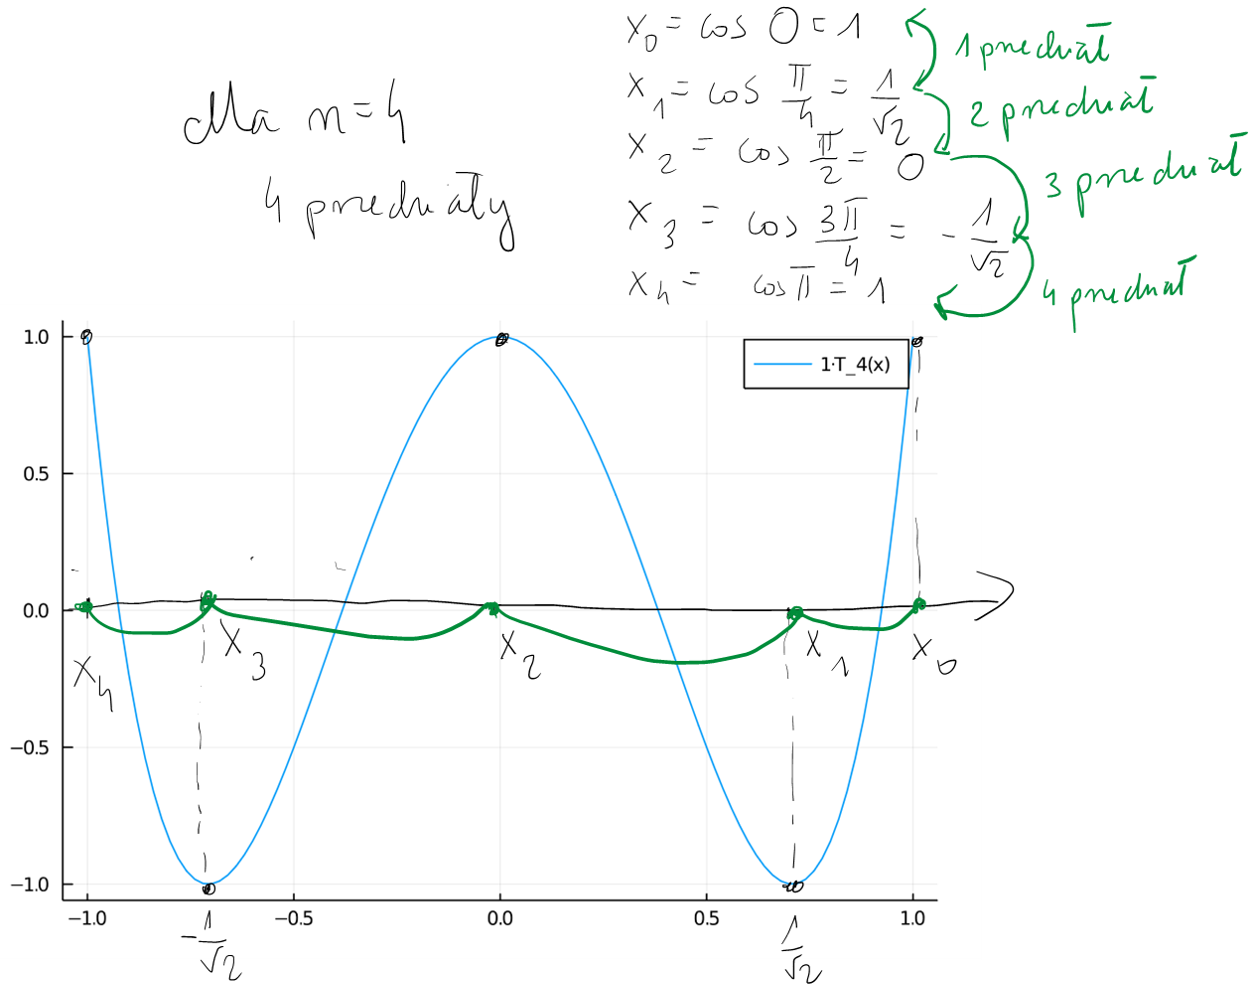
\includegraphics[height=0.82\textheight]{img/5/czeb.png}
	\end{figure}
\end{frame}
%%%%%%%%%%%%%%%%%%%
\begin{frame}
		$x'_k$ jest punktem ekstremalnym jeśli $T_n(x'_k)=(-1)^k$,\\
		analogicznie jak dla przypadku miejsc zerowych zachodzi:\\ $x_k'=\cos\frac{k\pi}{n}$, $k=0,1,.,n$\\
        Dla $\forall x_k'$ powinno zachodzić: \\
        $p_n(x_0') < 2^{1-n} \cdot T_n(x_0')$, \\
        $p_n(x_1') > 2^{1-n} \cdot T_n(x_1')$, \\
        $p_n(x_2') < 2^{1-n} \cdot T_n(x_2')$, \\
        \ldots , aż do $x_n'$ \\
        $\Rightarrow$ czyli wielomian $[p_n(x) - 2^{1-n} \cdot T_n(x)]$ \\
        powinien zmieniać znak w każdym z przedziałów: \\
        $(x_{k+1}',x_k')$, $k = \underbrace{n-1, n-2,..,1,0}_{\text{n przedziałów $\rightarrow$ n zer}} $\\ 
         $\Rightarrow $ czyli powinien być wielomianem stopnia $n$ w $[-1,1]$, \\ 
         ale $p_n(x)$ i $2^{1-n} \cdot T_n(x)$ mają ten sam współczynnik wiodący, \\
         Zatem ich różnica jest stopnia $n-1$ i mamy sprzeczność.
	
\end{frame}
%%%%%%%%%%%%%%%%%%%
\begin{frame}{Interpolacja  węzłami $T_{n+1}(x)$}
	$W_n(x)$ - wielomian interpolacyjny (Lagrange'a) stopnia $n$; $W_n(x_k) = f(x_k),k=0,1,..,n$
	Ze wzoru na błąd interpolacji Lagrange'a mamy:
    $$f(x) = W_n(x)+E_n(x); E_n(x) = \frac{f^{(n+1)}(c)}{(n+1)!}\underbrace{\prod_{i=0}^{n}(x-x_i)}_{\omega_{n+1}}
	, c \in [x_0,x_n]$$
    Przez optymalny wybór rozmieszczenia węzłów $x_k$ można zminimalizować $max|\omega_{n+1}(x)|$\newline
    \end{frame}
    \begin{frame}
   \textbf{Rozwiązanie:} Wprost z własności minimaksu - wielomianem mającym najmniejszy $max|\omega_{n+1}(x)|$ jest $2^{-n} \cdot T_{n+1}(x)$, który możemy przedstawić przy pomocy jego zer $x_i$ jako:
   $$2^{-n}\cdot T_{n+1}(x)=\prod_{i=0}^{n}(x-x_i)$$
    Czyli jako węzły interpolacji należy wziąć zera wielomianu $T_{n+1}(x)$
    $$x_k = \cos \Big(\frac{2k+1}{n+1}\frac{\pi}{2}\Big), k=0,1,..,n $$
    
\end{frame}
%%%%%%%%%%%%%%%
\begin{frame}
    \begin{block}{Uwaga}
        Transformacja przedziału $x \in [a,b] \rightarrow t \in [-1,1]$
        $$x=\frac{b-a}{2}t+\frac{a+b}{2}$$
    \end{block}
    Na następnych slajdach porównanie:\\
     - interpolacja z równoodległymi węzłami (11 węzłów)\newline
    - interpolacja z węzłami Czebyszewa $\rightarrow$ zera $T_{11}(x)$
\end{frame}
%%%%%%%%%%%%%%%%%%%
\begin{frame}
    \begin{figure}
        \includegraphics[height=0.8\textheight]{img/5/czebyszew.jpg}
    \end{figure}
\end{frame}
%%%%%%%%%%%%%%%%%%%
\begin{frame}
    \begin{figure}
        \includegraphics[height=0.8\textheight]{img/5/interpolacja.jpg}
    \end{figure}
\end{frame}
%%%%%%%%%%%%%%%%%%%
%%%%%%%%%%%%%%%%%%%
\begin{frame}{Interpolujący wielomian Czebyszewa}
	$T_n(x)$ zachowują się równomiernie w $[-1,1]$; min = -1, max = 1 - \textbf{ważna własność} \newline
    Do utworzenia wielomianu interpolacyjnego można wykorzystać liniową kombinację:
    $$W_n(x) = \sum_{j=0}^{n}c_jT_j(x)$$
    Współczynniki $c_j$ wyznaczamy  z własności ortogonalności dla przypadku dyskretnego:\\
    Jeśli $x_k=\cos\Big(\frac{2k+1}{n+1}\frac{\pi}{2}\Big)  \text{są zerami } T_{n+1}(x), k=0,1,..,n$ to:\\
    $\sum_{k=0}^{n}T_i(x_k)T_j(x_k) = \left\{\begin{array}{cc}
    	0 & i \not= j \\
        n+1 & i=j=0 \\
        \frac{n+1}{2} & i=j\not=0
    \end{array}\right.$$
\end{frame}
%%%%%%%%%%%%%%%%%%%
\begin{frame}{Wyznaczanie współczynników $c_i$}
Korzystamy z warunku interpolacji:
	$$f(x_k)= \sum_{j=0}^{n}c_jT_j(x_k)$$
	Następnie dla każdego węzła mnożymy ten warunek obustronnie przez $T_i(x_k)$ i składamy je w sumę:
	$$f(x_k)= \sum_{j=0}^{n}c_jT_j(x_k)\Bigg\arrowvert T_i(x_k)) \Bigg\arrowvert \sum_{k=0}^{n}$$
    $$\sum_{k=0}^{n}f(x_k)T_i(x_k)=\sum_{j=0}^{n}c_j\underbrace{\sum_{k=0}^{n}T_i(x_k)T_j(x_k)}_{\text{ortogonalność}}$$
\end{frame}
%%%%%%%%%%%%%%%%%%%
\begin{frame}{Współczynniki $c_i$}
Z warunku ortogonalności znikają wszystkie składniki $\sum_{j=0}^{n}$ poza $j=i$ i mamy:
 $$\sum_{k=0}^{n}f(x_k)T_i(x_k)=c_i\underbrace{\sum_{k=0}^{n}T_i(x_k)T_i(x_k)}_{\text{ortogonalność}}$$
 $\sum_{k=0}^{n}f(x_k)T_0(x_k)=c_0(n+1)$ czyli 
 $c_0 = \frac{1}{n+1}\sum_{k=0}^{n}f(x_k)T_0(x_k)$\\
 \vspace{0.5cm}
 $\sum_{k=0}^{n}f(x_k)T_i(x_k)=c_i\frac{n+1}{2}$ czyli
 $c_i = \frac{2}{n+1}\sum_{k=0}^{n}f(x_k)T_i(x_k)$\\
 dla $ i=1,..,n$\\
 Wspólczynniki są od siebie niezależne ! (pomocny: alg. Clenshawa)\\
Jeśli wyliczymy ich mniej - aproksymacja. Porównaj (slajd 17) 
$$\sum_{i=0}^{n}w(x_i)F(x_i)\varphi_k(x_i)=a_k\sum_{i=0}^{n}w(x_i)\varphi_k^2(x_i)$$
\end{frame}
\begin{frame}{Analogia do wektorów $R^2$}
    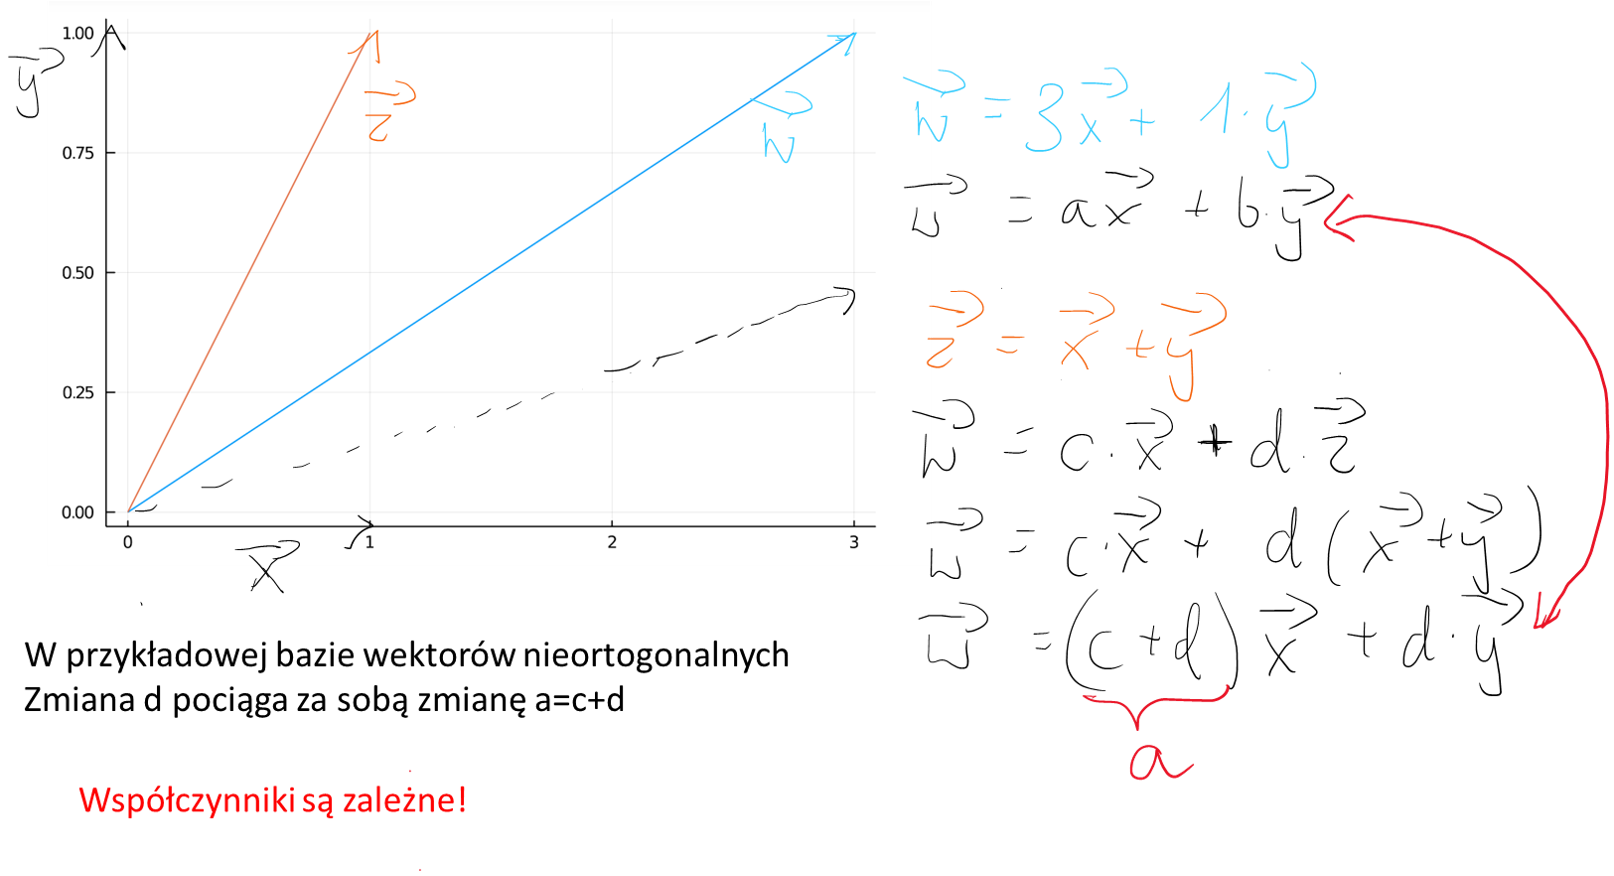
\includegraphics[height=0.7\textheight]{img/5/ortovsnieorto.png}
\end{frame}
\begin{frame}{Szacowanie błędu aproksymacji}
Maksymalna odległość między "kolejnymi" aproksymacjami w bazie wielomianów Czebyszewa liczona przy użyciu normy aproksymacii jednostajnej $sup_{x \in [a,b]}|g(x)-f(x)|$ to:
    $$f(x)=a_n\cdot T_{n}(x)+a_{n-1}\cdot T_{n-1}(x)+...+a_1\cdot T_{1}(x)+a_0\cdot T_{0}(x)$$
     $$g(x)=a_{n-1}\cdot T_{n-1}(x)+...+a_1\cdot T_{1}(x)+a_0\cdot T_{0}(x)$$
     $$|g(x)-f(x)|< |a_n|\cdot \underbrace{|T_{n}(x)|}_{max 1}\le |a_n|$$
     Kolejne współczynniki mówią nam o błędach przybliżenia!\\
     Jeśli współczynniki wyższych rzędów maleją $\rightarrow$ wskaźnik, że funkcja "nadaje się" do aproksymacji wielomianami.\\
    
\end{frame}
\begin{frame}{Co przy pomiarach?}
     Problem:  Trzeba znać wartości funkcji aproksymowanej w węzłach Czebyszewa.\\
Możliwe (alternatywne) rozwiązania:
\begin{itemize}
    \item mierzyć w węzłach Czebyszewa
    \item     mierzyć wystarczająco  gęsto
    \item użyć aproksymacji wielomiami Czebyszewa w "złych" punktach, ale z dobranymi wagami mówiącymi o jakości tych punktów. 
\end{itemize}
\end{frame}
%%%%%%%%%%%%%%%%%%%
\begin{frame}{Aproksymacja wielomianami Czebyszewa (p. ciągły)}
    Aproksymacja jednostajna: $minsup_{x \in [a,b]}|F(x)-f(x)|$ \newline
    Baza $T_i(x)$ wygodna, bo $T_i(x)$ - równomierne w $[-1,1]$ \\
    \vspace{0.5cm}
    Pierwszy sposób (podobnie jak w metodzie  szeregów potęgowych):
    $F(x)$ \textbf{zastępujemy sumą częściową:}
    $$F(x) \approx \sum_{j=0}^{n}c_jT_j(x)$$
    z $c_j$ wyznaczonymi z warunku ortogonalności w przypadku ciągłym
    $$F(x) = \sum_{j=0}^{\infty}c_jT_j(x)    \bigg\arrowvert \cdot\frac{T_i(x)}{\sqrt{1-x^2}}  \bigg\arrowvert \int_{-1}^{1}dx$$
    \begin{tabular}{ll}
        $c_0 = \frac{1}{\pi}\int_{-1}^{1}\frac{F(x)T_0(x)dx}{\sqrt{1-x^2}}$ &
        $c_i = \frac{2}{\pi}\int_{-1}^{1}\frac{F(x)T_i(x)dx}{\sqrt{1-x^2}}, i=1,..,n$
    \end{tabular}

\end{frame}
%%%%%%%%%%%%%%%%%%%
\begin{frame}
    Drugi sposob analogiczny do aproksymacji Pade.\\ Tworzymy wyrażenia wymierne postaci:
    $$T_{n,k}(x) = \frac{\sum_{i=0}^{n}a_iT_i(x)}{\sum_{i=0}^{k}b_iT_i(x)}$$
    o $a_i$, $b_i$ dobranych tak, licznik wyrażenia  
     $$F(x)-T_{n,k}(x) = \frac{\big[\sum_{j=0}^{\infty}c_jT_j(x)\big] \cdot \big[\sum_{i=0}^{k}b_iT_i(x)\big] - \sum_{i=0}^{n}a_iT_i(x)}{\sum_{i=0}^{k}b_iT_i(x)}$$
     był równy  kombinacji liniowej wielomianów Czebyszewa o wskaźnikach większych od k+n. \\
     
     Dla zainteresowanych:
    \url{https://pl.wikibooks.org/wiki/Metody_numeryczne_fizyki/Aproksymacja}
\end{frame}
